%%%%%%%% ICML 2025 EXAMPLE LATEX SUBMISSION FILE %%%%%%%%%%%%%%%%%

% STRICT 4-PAGE LIMIT!!

\documentclass{article}

% Recommended, but optional, packages for figures and better typesetting:
\usepackage{microtype}
\usepackage{graphicx}
\usepackage{subfigure}
\usepackage{booktabs} % for professional tables
\usepackage{tabularx}

% hyperref makes hyperlinks in the resulting PDF.
% If your build breaks (sometimes temporarily if a hyperlink spans a page)
% please comment out the following usepackage line and replace
% \usepackage{icml2025} with \usepackage[nohyperref]{icml2025} above.
\usepackage{hyperref}


% Attempt to make hyperref and algorithmic work together better:
\newcommand{\theHalgorithm}{\arabic{algorithm}}

% Use the following line for the initial blind version submitted for review:
% \usepackage{icml2025}

% If accepted, instead use the following line for the camera-ready submission:
\usepackage[accepted]{icml2025}


%--------------------------------------
% FONT SETUP FOR XeLaTeX WITH ANCIENT GREEK
%--------------------------------------
\usepackage{fontspec} % for XeLaTeX
\setmonofont{DejaVu Sans Mono}[Scale=MatchLowercase] % English font

% Main fonts
\setmainfont{NewComputerModern10}                % main text
%\setmonofont{DejaVu Sans Mono}[Scale=0.8]       % monospace

% Ancient Greek font
\newfontfamily\greekfont[%
    Path=fonts/,
    UprightFont = *,        % main upright style
    BoldFont = GFSDidotBold.otf,
    ItalicFont = GFSDidotItalic.otf,
    Script = Greek,         % necessary for polyglossia
    Scale = MatchLowercase
]{GFSDidot.otf}
\newfontfamily\greekfontsf[%
    Path=fonts/,
    UprightFont = *,        % main upright style
    BoldFont = GFSDidotBold.otf,
    ItalicFont = GFSDidotItalic.otf,
    Script = Greek,         % necessary for polyglossia
    Scale = MatchLowercase
]{GFSDidot.otf}
\newfontfamily\kadmosu[
    Path = fonts/,            
    Extension = .ttf,         
    UprightFont = KadmosU
]{KadmosU}

% Polyglossia
\usepackage{polyglossia}
\setdefaultlanguage{english}
\setotherlanguage[variant=ancient]{greek}

%--------------------------------------
% END FONT SETUP FOR XeLaTeX
%--------------------------------------

% For theorems and such
\usepackage{amsmath}
\usepackage{amssymb}
\usepackage{mathtools}
\usepackage{amsthm}

% if you use cleveref..
\usepackage[capitalize,noabbrev]{cleveref}

%%%%%%%%%%%%%%%%%%%%%%%%%%%%%%%%
% THEOREMS
%%%%%%%%%%%%%%%%%%%%%%%%%%%%%%%%
\theoremstyle{plain}
\newtheorem{theorem}{Theorem}[section]
\newtheorem{proposition}[theorem]{Proposition}
\newtheorem{lemma}[theorem]{Lemma}
\newtheorem{corollary}[theorem]{Corollary}
\theoremstyle{definition}
\newtheorem{definition}[theorem]{Definition}
\newtheorem{assumption}[theorem]{Assumption}
\theoremstyle{remark}
\newtheorem{remark}[theorem]{Remark}

% Todonotes is useful during development; simply uncomment the next line
%    and comment out the line below the next line to turn off comments
%\usepackage[disable,textsize=tiny]{todonotes}
\usepackage[textsize=tiny]{todonotes}


% The \icmltitle you define below is probably too long as a header.
% Therefore, a short form for the running title is supplied here:
\icmltitlerunning{Papyrus Imputation Topics}

% Mina custom-spaket
\usepackage{epigraph}

% Stan code: listings with a small Stan language definition
\usepackage{listings}
\usepackage{tikz}
\usetikzlibrary{shapes.geometric,arrows.meta,positioning,calc}
\lstdefinelanguage{Stan}{
  morekeywords={data,transformed,parameters,model,generated,quantities,
    functions,for,in,if,else,while,target,return,print,reject},
  morekeywords=[2]{int,real,vector,row_vector,matrix,simplex,array,
    unit_vector,ordered,positive_ordered,cov_matrix,corr_matrix,lower,upper},
  morekeywords=[3]{dirichlet,normal,gamma,beta,multinomial,categorical,
    rep_vector,log,exp,log_sum_exp,sum,softmax},
  sensitive=true,
  morecomment=[l]{//},
  morecomment=[s]{/*}{*/},
}
\lstset{
  language=Stan,
  basicstyle=\ttfamily\footnotesize,
  keywordstyle=\bfseries\color{blue!60!black},
  keywordstyle=[2]\color{teal!70!black},
  keywordstyle=[3]\color{purple!70!black},
  commentstyle=\itshape\color{gray},
  columns=fullflexible,
  keepspaces=true,
  breaklines=true,
  frame=single,
  framerule=0.3pt,
  rulecolor=\color{gray!60},
  aboveskip=1ex,
  belowskip=1ex,
}

\begin{document}

\twocolumn[
\icmltitle{Modelling the Topics of Machine-Generated Imputations for an Ancient Greek Papyrus}

% It is OKAY to include author information, even for blind
% submissions: the style file will automatically remove it for you
% unless you've provided the [accepted] option to the icml2025
% package.

% List of affiliations: The first argument should be a (short)
% identifier you will use later to specify author affiliations
% Academic affiliations should list Department, University, City, Region, Country
% Industry affiliations should list Company, City, Region, Country

% You can specify symbols, otherwise they are numbered in order.
% Ideally, you should not use this facility. Affiliations will be numbered
% in order of appearance and this is the preferred way.
\icmlsetsymbol{equal}{*}

\begin{icmlauthorlist}
\icmlauthor{Albin Thörn Cleland}{yyy}
% \icmlauthor{Firstname2 Lastname2}{equal,yyy,comp}
% \icmlauthor{Firstname3 Lastname3}{comp}
% \icmlauthor{Firstname4 Lastname4}{sch}
% \icmlauthor{Firstname5 Lastname5}{yyy}
% \icmlauthor{Firstname6 Lastname6}{sch,yyy,comp}
% \icmlauthor{Firstname7 Lastname7}{comp}
%\icmlauthor{}{sch}
% \icmlauthor{Firstname8 Lastname8}{sch}
% \icmlauthor{Firstname8 Lastname8}{yyy,comp}
%\icmlauthor{}{sch}
%\icmlauthor{}{sch}
\end{icmlauthorlist}

\icmlaffiliation{yyy}{Swedish Graduate School of Digital Philology, Centre for Languages and Literature, The Joint Faculties of Humanities and Theology, Lund University, Lund, Sweden}
% \icmlaffiliation{comp}{Company Name, Location, Country}
% \icmlaffiliation{sch}{School of ZZZ, Institute of WWW, Location, Country}

\icmlcorrespondingauthor{Albin Thörn Cleland}{albin.thorn\_cleland@klass.lu.se}
% \icmlcorrespondingauthor{Firstname2 Lastname2}{first2.last2@www.uk}

% You may provide any keywords that you
% find helpful for describing your paper; these are used to populate
% the "keywords" metadata in the PDF but will not be shown in the document
\icmlkeywords{Multiple Imputation, Bayesian Data Analysis, Stan, NLP, Digital Philology, Ancient Greek, Papyrology, Text Restoration}

\vskip 0.3in
]

% this must go after the closing bracket ] following \twocolumn[ ...

% This command actually creates the footnote in the first column
% listing the affiliations and the copyright notice.
% The command takes one argument, which is text to display at the start of the footnote.
% The \icmlEqualContribution command is standard text for equal contribution.
% Remove it (just {}) if you do not need this facility.

\printAffiliationsAndNotice{}  % leave blank if no need to mention equal contribution
% \printAffiliationsAndNotice{\icmlEqualContribution} % otherwise use the standard text.

\begin{abstract}
We conduct the first large-scale evaluation of machine-generated imputations for a damaged Ancient Greek papyrus. A large number of conjectures are generated by a non-ergodic ``Metropolis-in-Gibbs'' random walk through the space of formally possible restorations. Even though the complete space is formally too large to explore due to combinatorial explosion, the joint restrictions of verse and semantic context make it plausible that topic modelling a large sample is still valuable information regarding the lost true topic. We compare the restorations' topics with Sophocles' under two models: hard topics, with an exact conjugate Dirichlet--multinomial posterior, and soft topics from a seeded latent Dirichlet allocation, whose posterior is sampled with NUTS one restoration at a time. 
\end{abstract}

\section{Introduction}
\label{introduction}

Conjectural text criticism is one of the most methodologically controversial parts of classical philology, but also one of the most well-established.\footnote{See \citet{olson2020tereus} for a recent critique of what the author sees as the shaky methodological foundation of conjectural text criticism.} Since Hellenistic times, scholars have made informed conjectures as to what the lacunae of damaged or corrupted texts could have said, conjectures that are sometimes vindicated or falsified by newly found papyri. Large masked-language models (MLM) like \citet{cullhed2026stoicheiacharacterlevelmaskeddiffusion} hold the promise to let scholars avoid criticisms of subjectivity and anachronism by shifting the basic method from the ingenuity of individual editors (what \citet{conte2013ope} calls \textit{ope ingenii}) to statistical treatments of large arrays of machine generated conjectures. With this radical change of method, the research question changes from ``is this particular reconstruction probable'' to ``how probable is it that the true reconstruction is somewhere among these $N$ machine reconstructions'', given very large-dimensional stylometric feature vectors for them and a set of strongly informative priors regarding the distribution of characteristics of the extant corpus. 

As a case study, we use the famous papyrus \textit{P.Oxy 5292} first published in \citet{slattery2016tereus} (see \autoref{papyrus}), which preserves a fragmentary continuation of a preserved quote from Sophocles' otherwise lost play \textit{Tereus}, a staging of the myth of Philomela. 

% \epigraph{[I]dentifying the point at which "same" turns into "different" is a fundamentally subjective enterprise.}{Olson, \emph{Methodological Reflections on the Text and Action of Sophocles' \emph{Tereus}}, p.\ 184}
% \epigraph{Some people ask "Who is to be the official guesser of priors?" and "Won't different people get different results?." The answers are "No one," and "Yes."}{Mosteller and Wallace, p.\ 303}

\section{Research questions}
\label{questions}

Let us in this context define a `topic' as a probability distribution over a set vocabulary of lemmata (the normalized and uninflected dictionary form a given word token is marked as belonging to by a lemmatizer). That a certain topic $t$ `stands out' in a corpus of texts or windows of texts is then defined as the posterior probability that its mean lemma rates are closer to $t$ than the rates of some baseline are. 

We are now ready to ask: are there topics that consistently stand out across chains and iterations of generated papyrus imputations? 

\section{Data}
\label{data}

The imputations come from a judge-steered Metropolis walk over restorations
of the seventeen damaged verses (vv.~13--29): the character-level diffusion
model Stoicheia proposes a replacement for a short span, formal metrical and
orthographic rules filter it, and an open-weight LLM judge\footnote{Qwen3-235B-A22B-Instruct-2507,
\url{https://huggingface.co/Qwen/Qwen3-235B-A22B-Instruct-2507}.}
accepts or rejects it by a Metropolis--Hastings step (\autoref{walk}).
Sixteen chains start from eight reconstructions by Eric Cullhed, and a state is
recorded every ten steps after a burn-in of 300, giving 17\,120 restorations.
Every text is lemmatised and reduced to a bag of lemmata over a vocabulary of
3\,128 lemmata.

A \textbf{document} is one whole restoration of the seventeen verses, on
average 26 topic-bearing lemmata; only restored text counts, never the
surviving letters. The baseline is Sophocles himself: his extant trimeters,
cut into 444 windows of seventeen consecutive verses, the shape of the
lacuna. Two further baselines tell what is unsophoclean from what is merely
untragic: Aeschylus and Euripides (1\,174 windows) and Classical Attic, the
Attic authors before Alexander (23\,328 windows), both in windows of 30
lemmata.

\section{Models and methods}
\label{models}

\subsection{Hard topics: conjugate posterior}

Every lemma of the vocabulary belongs to exactly one of 34 semantic clusters
(Word2Vec, \citealt{mikolov2013efficient}, on the lemmatised Greek corpus,
Ward's method cut at $K = 40$, two rare-lemma and four function-word clusters
dropped), named by the English glosses of the three non-cognate lemmata
nearest its centroid, for example \textit{lament-pitiable-groan}
(\cref{tab:topics}). A document's topic counts $\mathbf n$ are then
\[\mathbf n \mid \theta \sim \mathrm{Multinomial}(N, \theta), \qquad
  \theta \sim \mathrm{Dirichlet}(\kappa \mathbf m),\]
where $N$ is the document's own length, $\mathbf m$ is Sophocles' topic
profile and $\kappa = 1$: a restoration is a priori Sophoclean, but the prior
is worth a single lemma, so a document of twenty lemmata is 95\,\% data. A
symmetric prior would pull short documents towards the uniform profile and
so fabricate lift for topics they simply lack. The posterior
$\theta \mid \mathbf n \sim \mathrm{Dirichlet}(\kappa \mathbf m + \mathbf n)$
is exact and is sampled by normalised gamma draws.

\subsection{Soft topics: MCMC posterior}

Hard clusters put every occurrence of a lemma into one topic, although a
frequent word can serve several. The soft model gives each topic a
distribution $\phi_k$ over the vocabulary (\cref{fig:phi}), fitted once by a seeded
latent Dirichlet allocation \citep{blei2003latent} on Aeschylus and Euripides
only (tomotopy, \citealt{lee2022tomotopy}),\footnote{In LDA each
document $d$ has topic shares $\theta_d \sim \mathrm{Dirichlet}(\alpha)$ and
each topic a word distribution $\phi_k \sim \mathrm{Dirichlet}(\beta_k)$;
every lemma token first draws a topic $z \sim \theta_d$, then the lemma from
$\phi_z$. Tomotopy fits this by collapsed Gibbs sampling: $\theta$ and $\phi$
are integrated out, each token's topic is redrawn in turn given all the
others (1\,000 sweeps), and $\phi_{k,w} \propto n_{k,w} + \beta_{k,w}$ is read
off the final counts $n$. Seeding changes only the prior: a lemma of
cluster $k$ has $\beta_{k,w} = 200$, two hundred pseudo-occurrences in its own
topic, and $0.01$ in every other, while unclustered lemmata and the four free
topics get $0.01$ throughout. Here $\alpha = 0.1$, $K = 38$, and the documents
are the 1\,174 windows of Aeschylus and Euripides.} so that Sophocles is a test corpus
like the restorations. Each hard cluster seeds one topic with a strong prior
on its lemmata, and four free topics take up what the clusters miss.
\textgreek{θεός}, god, which the hard model puts in \textit{god-true-lord}
alone, is now split between two topics: given the word, the free topic
\textit{god-word-do} has probability 0.80 and \textit{god-true-lord} 0.18
($\phi_{k,w}$ normalised over $k$). With
$\phi$ fixed, a document's lemmata are drawn from the mixture
$\sum_k \theta_k \phi_k$ with $\theta \sim \mathrm{Dirichlet}(\mathbf 1)$, and
the posterior
\[p(\theta \mid w_{1:N}) \propto \prod_{n=1}^{N} \sum_{k=1}^{K}
  \theta_k\, \phi_{k w_n}\]
has no closed form. It is sampled with NUTS in Stan
\citep{carpenter2017stan}, one document at a time, by the program shown in the
frame (diagnostics in \autoref{diagnostics}).

\begin{figure}[t]
\centering
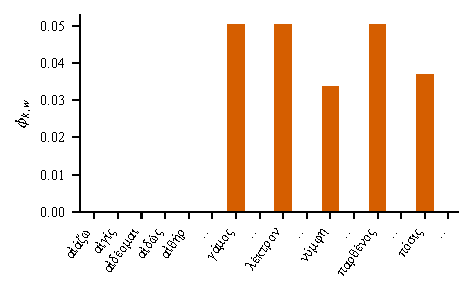
\includegraphics[width=\linewidth]{figures/phi_marriage.pdf}
\caption{Part of $\phi_k$ for \textit{marriage-couch-bed}, lemmata in
vocabulary order. Most of the 3,128 lemmata, like the first five, get about
$3\cdot10^{-5}$; the mass sits on a few, such as \textgreek{γάμος} and
\textgreek{λέκτρον}, marriage and the marriage bed.}
\label{fig:phi}
\end{figure}

\begin{lstlisting}[float=tp]
data {
  int<lower=1> N;
  int<lower=1> K;
  matrix[N, K] logphi; // log phi[:, w_n] for each lemma
}
parameters {
  simplex[K] theta;
}
model {
  // prior
  theta ~ dirichlet(rep_vector(1, K));

  // likelihood
  vector[K] log_theta = log(theta);
  for (n in 1:N)
    target += log_sum_exp(log_theta + logphi[n]');
}
\end{lstlisting}

\subsection{Comparing the imputations with Sophocles}

A set of documents gives two posteriors. The \textbf{mean profile}
$\bar\theta$ averages the documents' posteriors draw by draw and says what
the imputations put into the lacuna on average. The \textbf{random document}
is the equal mixture of the documents' posteriors; set against a random
Sophoclean window, $P(\theta_k^{\text{doc}} > \theta_k^{\text{window}})$
measures how far the two populations overlap (0.5 if not at all apart). The
\textbf{lift} of topic $k$ is the ratio of the imputations' mean share to
Sophocles', and a topic is \textbf{raised} when its lift is at least 1.5 and
$P(\bar\theta_k^{\text{imp}} > \bar\theta_k^{\text{Soph}}) \ge 0.9$. The
restorations are not independent, since successive states of a chain share
most of their words; the hard model's 90\,\% intervals for a lift therefore
resample whole chains (and Sophocles by window), while the soft model's come
from the posterior draws alone and are too narrow.

\section{Results}
\label{results}

\begin{figure}[!t]
\centering
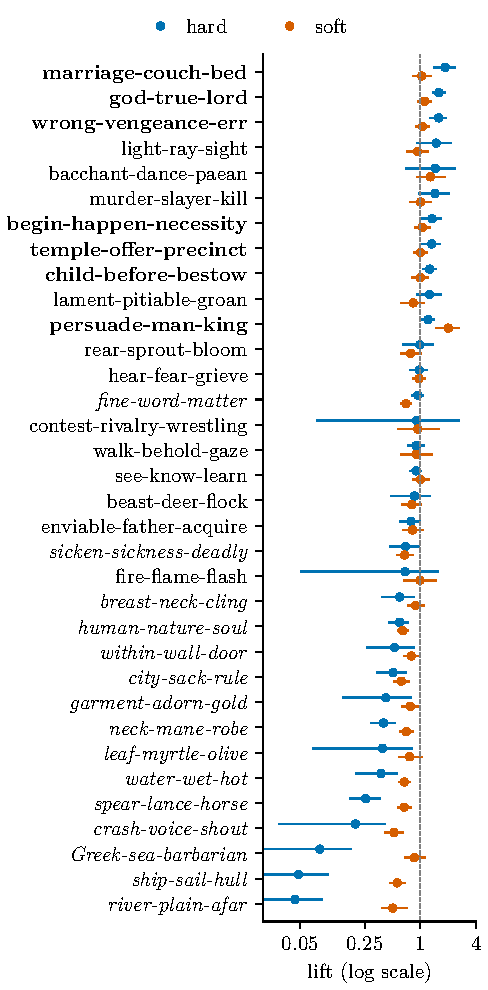
\includegraphics[width=\linewidth]{figures/lift_hard_soft.pdf}
\caption{Lift of the imputations against Sophocles for every topic, with
90\,\% intervals (hard: resampled by chain; soft: posterior draws). Dashed: no
difference; dotted: the lift of 1.5 that counts as raised.}
\label{fig:lift}
\end{figure}

\begin{table}[t]
\centering
\scriptsize
\setlength{\tabcolsep}{3pt}
\begin{tabular}{lrrrrrr}
\toprule
 & \multicolumn{3}{c}{hard} & \multicolumn{3}{c}{soft} \\
\cmidrule(lr){2-4}\cmidrule(lr){5-7}
Topic & Soph. & A.\,\&\,E. & Attic & Soph. & A.\,\&\,E. & Attic \\
\midrule
wrong-vengeance-err & 1.58 & 1.49 & 1.61 & 1.18 & 1.17 & 1.08 \\
god-true-lord & 1.59 & 1.89 & 1.48 & 1.16 & 1.32 & 0.99$^\circ$ \\
marriage-couch-bed & 1.85 & 0.79 & 2.97 & 1.22 & 0.98$^\circ$ & 1.20 \\
persuade-man-king & 1.21 & 1.19 & 1.04$^\circ$ & 1.63 & 1.65 & 1.12 \\
\bottomrule
\end{tabular}
\caption{Lift of the imputations against the three baselines (Sophocles,
Aeschylus and Euripides, Classical Attic). $^\circ$: the 90\,\% interval
includes 1.}
\label{tab:key}
\end{table}

\paragraph{Hard topics.} The imputations write tragedy: of nine genres their
topic profile is nearest to tragedy (Jensen--Shannon divergence 0.044 bits,
against 0.082 for comedy and 0.150 for epic). It is not, however,
Sophocles' profile (\cref{fig:lift}). Five topics are raised:
\textit{marriage-couch-bed} (lift 1.83), \textit{god-true-lord} (1.56),
\textit{wrong-vengeance-err} (1.55), \textit{bacchant-dance-paean} and
\textit{light-ray-sight} (both 1.51), though the last two have intervals that
include 1 once whole chains are resampled. The deficits are deeper than the
excesses: the sea, rivers and Greeks against barbarians almost vanish
(\textit{ship-sail-hull} 0.05, \textit{river-plain-afar} 0.04,
\textit{Greek-sea-barbarian} 0.08).

The further baselines separate the unsophoclean from the untragic
(\cref{tab:key}).
\textit{god-true-lord} and \textit{wrong-vengeance-err} hold against all
three, every interval above 1 (lifts 1.48--1.89).
\textit{marriage-couch-bed} is raised against Sophocles (1.85) and Classical
Attic (2.97) but falls below Aeschylus and Euripides (0.79, interval
0.61--0.98), who use that vocabulary more than Sophocles does. Lemma by
lemma, the excess of \textit{god-true-lord} is a single word: \textgreek{θεός}
occurs 43.9 times per thousand topic lemmata in the restorations against 15.6
in Sophocles. That of \textit{wrong-vengeance-err} is spread over the matter
of the play: \textgreek{χάρις}, \textgreek{πόνος}, \textgreek{δίκη}, \textgreek{πάθος} and \textgreek{τιμωρός}, favour,
toil, justice, suffering and the avenger.

Individually the restorations are much less distinctive than their average.
For every topic a random restoration exceeds a random Sophoclean window with
probability between 0.37 and 0.66: even the raised topics only tilt a
population that overlaps heavily with Sophocles'.

\paragraph{Soft topics.} Under the soft model the lifts shrink towards 1
(range 0.83--1.63) and only \textit{persuade-man-king} is raised (1.63,
interval 1.54--1.76). \textit{god-true-lord} falls to 1.16 and
\textit{marriage-couch-bed} to 1.22. The reason is visible in $\phi$: the most
frequent words of tragedy leave their clusters for the free topics, as
\textgreek{θεός} does for \textit{god-word-do}, so the hard model's excess of \textgreek{θεός} is no longer an excess of the
god topic. \textit{wrong-vengeance-err} is the one raised topic of the hard
model that stays above all three baselines under the soft model too (lifts
1.18, 1.17 and 1.08).

\paragraph{Robustness.} Eight chains from deliberately unrelated starts give
a hard profile whose log lifts correlate at 0.76 with the main set's;
\textit{god-true-lord} stays raised and \textit{wrong-vengeance-err} keeps a
lift of 1.45 (1.38--1.54). The judge matters more: a pilot with Claude Sonnet
5.5 as judge correlates with the Qwen profile at only 0.30, yet
\textit{persuade-man-king} and \textit{wrong-vengeance-err} stay above
Sophocles. Single chains differ widely, the lift of
\textit{wrong-vengeance-err} ranging from 0.74 to 3.00 over the sixteen
chains, so the pooled profile is an average over chains that have not mixed;
the chain-resampled intervals carry that uncertainty (\autoref{diagnostics}).

\section{Conclusions}
\label{conclusions}


\section{Data availability statement}

The imputations, the baseline windows, the vocabulary and topics, and the
soft model's $\phi$ and posterior draws are on Hugging Face at
\url{https://huggingface.co/datasets/Urdatorn/bsda-miniproject-2026}. The
code for the models, the reports and this paper is on GitHub at
\url{https://github.com/Urdatorn/bsda-miniproject-2026}.

\section{Acknowledgements}

This experiment was carried out under the aegis of a long-term research program launched in 2024 by Eric Cullhed and titled \textit{Dionysus Recomposed. A Modular Approach to Restoring Ancient Tragic Fragments with Machine Learning}, as an application and refinement of \citet{cullhed2026stoicheiacharacterlevelmaskeddiffusion}. Using the \textit{Tereus} fragment as a pilot test was suggested by Cullhed.

\bibliography{bsda}
\bibliographystyle{icml2025}


%%%%%%%%%%%%%%%%%%%%%%%%%%%%%%%%%%%%%%%%%%%%%%%%%%%%%%%%%%%%%%%%%%%%%%%%%%%%%%%
%%%%%%%%%%%%%%%%%%%%%%%%%%%%%%%%%%%%%%%%%%%%%%%%%%%%%%%%%%%%%%%%%%%%%%%%%%%%%%%
% APPENDIX
%%%%%%%%%%%%%%%%%%%%%%%%%%%%%%%%%%%%%%%%%%%%%%%%%%%%%%%%%%%%%%%%%%%%%%%%%%%%%%%
%%%%%%%%%%%%%%%%%%%%%%%%%%%%%%%%%%%%%%%%%%%%%%%%%%%%%%%%%%%%%%%%%%%%%%%%%%%%%%%
\newpage
\appendix
\onecolumn

\section{The papyrus}
\label{papyrus}

P.Oxy 5292 \citep{slattery2016tereus}. The first three lines of the right column overlap with the end of a section of Sophocles' \textit{Tereus} preserved by Stobaeus, which is how we know the context of the otherwise lost lines that follow.

\begin{center}
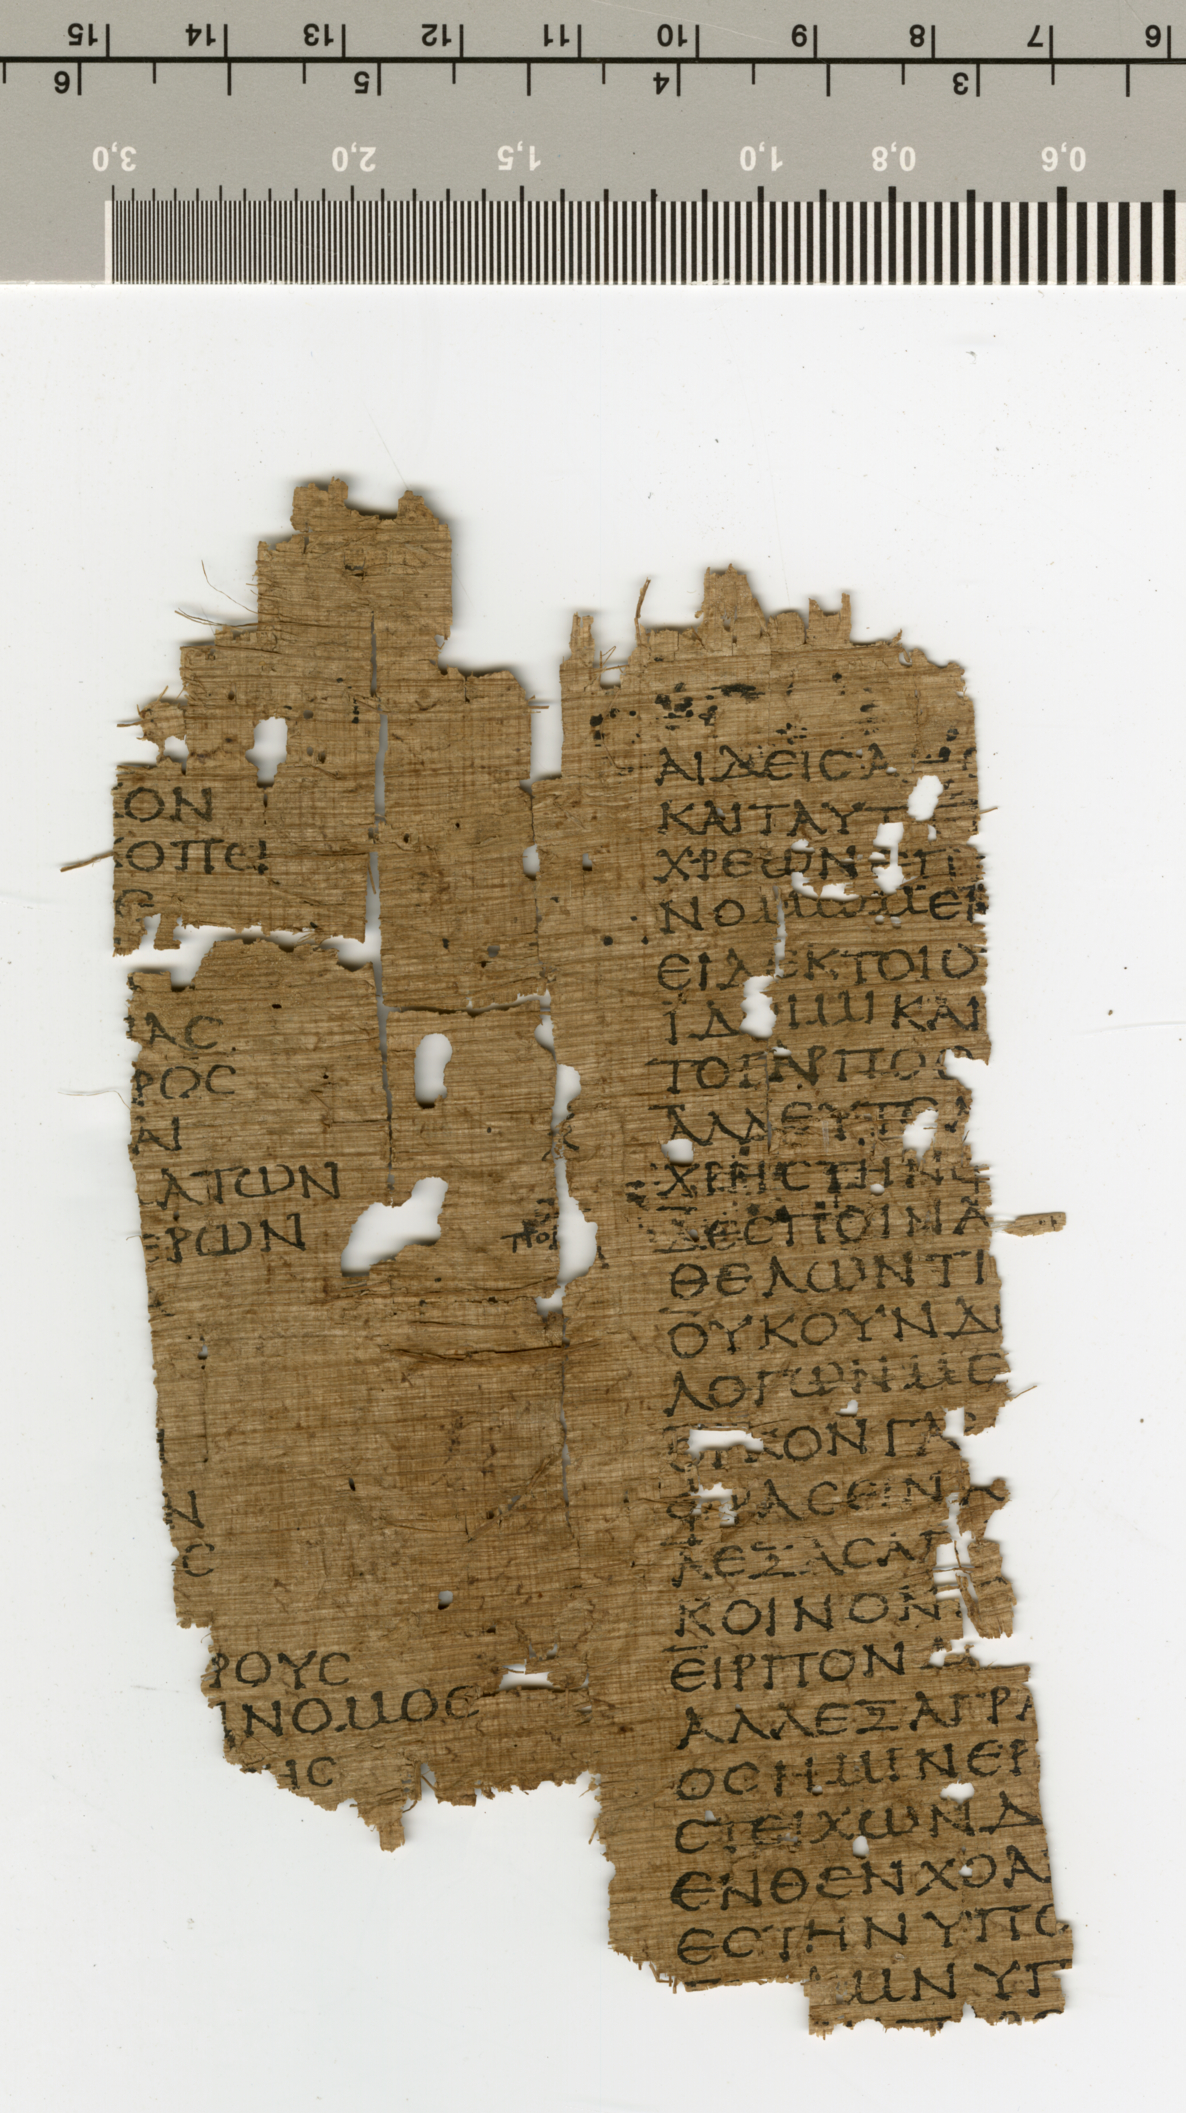
\includegraphics[height=0.75\textheight,width=\linewidth,keepaspectratio]{figures/POxy5292.jpg}
\end{center}

\newpage
\section{Input to Stoicheia}

Stoicheia is the first imputation model for papyri that does not require inputting the exact number of characters missing. Instead one can input a desired span. In our case, a plausible span can easily be estimated using the mean length of equivalent verse lines in Sophocles' preserved plays, for which see \autoref{tab:trimeter-lengths}.

\begin{table*}[htbp]
  \centering
  \label{tab:trimeter-lengths}
  \begin{tabular}{lrrrrrc}
    \toprule
    Author    & $n$    & Mean  & SD   & Min & Max & Central 95\,\% \\
    \midrule
    Aeschylus &  1\,780 & 30.75 & 2.21 & 23 & 40 & 26--35 \\
    \textbf{Sophocles} &  7\,545 & 30.05 & 2.07 & 22 & 38 & 26--34 \\
    Euripides & 18\,198 & 30.36 & 2.09 & 23 & 40 & 26--35 \\
    \midrule
    Pooled    & 27\,523 & 30.30 & 2.10 & 22 & 40 & 26--35 \\
    \bottomrule
  \end{tabular}
  \caption{Letters per verse line of iambic trimeter in the three tragedians.}
\end{table*}

The content of the prompt sent to Stoicheia to infer an imputation then looks like the below: 

\label{tereus}
    \begin{verbatim}
    νυνδουδενειμιχωρισαλλαπολλακισ
    εβλεψαταυτηιτηνγυναικειανφυσιν
    ωσουδενεσμεναινεαιμενενπατροσ
    ηδιστονοιμαιζωμενανθρωπωνβιον
    τερπνωσγαραειπαιδασανοιατρεφει
    οτανδεσηβηνεξικωμεθεμφρονεσ
    ωθουμεθεξωκαιδιεμπολωμεθα
    θεωνπατρωιωντωντεφυσαντωναπο
    αιμενξενουσπροσανδρασαιδεβαρβαρουσ
    αιδεισαηθηδωμαθαιδεπιρροθα
    καιταυτεπειδανευφρονηζευξηιμια
    χρεωνεπαινεινκαιδοκεινκαλωσεχειν
    νομωιμεν[22±4]
    ειδεκτοιου[20±4]
    ιδοιμικαι[21±4]
    τογαρποθ[22±4]
    αλλευτελ[22±4]
    χρηστηνφ[22±4]
    δεσποινα[22±4]
    θελωντι[23±4]
    ουκουνδ[23±4]
    λογωνμε[23±4]
    ορκονγαρ[22±4]
    φρασεινα[22±4]
    λεξασα[24±4]
    κοινον[24±4]
    ειρπονμ[23±4]
    αλλεξαγρασ[20±4]
    οσημινερ[22±4]
    \end{verbatim}

\newpage
\section{The Metropolis walk}\label{walk}

The restorations are the states of a Metropolis-within-Gibbs walk over the
seventeen damaged verses; the chart below shows one step. The
character-level diffusion model Stoicheia
\citep{cullhed2026stoicheiacharacterlevelmaskeddiffusion} proposes new text for
a span of one verse, hard formal checks discard impossible candidates, and a
surviving candidate is accepted with probability $\min(1, r)$. The ratio $r$
has two parts: small calibration terms that bring the restorer's habits
(finite verbs, particles, word repetition) to Sophocles' rates, and an LLM
judge's preference for the more coherent of the old and the new line. Nothing
in the walk rewards Sophoclean style as such, so it remains a source of
imputations rather than a search for the most Sophoclean text.

Sixteen chains start from Eric Cullhed's eight reconstructions and run
10\,000 steps each; after a burn-in of 300 steps every tenth state is kept.
The chains do not mix within that budget (\autoref{diagnostics}).

\begin{center}
\begin{tikzpicture}[
  node distance=5mm,
  box/.style={draw, rounded corners=2pt, align=left, text width=110mm, inner sep=5pt, fill=white},
  model/.style={box, fill=blue!6},
  judge/.style={box, fill=orange!10},
  dec/.style={draw, diamond, aspect=2.6, align=center, inner sep=1.5pt, fill=white},
  arr/.style={-{Stealth[length=2mm]}, thick},
  lab/.style={fill=white, inner sep=1.5pt},
]
\node[box] (start) {\textbf{Start} from a restoration of vv.~13--29; vv.~1--12
  survive and stay fixed.};
\node[box, below=of start] (pick) {\textbf{Pick a site}: a damaged verse and a
  span of its restored letters, at random.};
\node[model, below=of pick] (sto) {\textbf{Stoicheia proposes} replacements for
  the masked span, conditioned on the whole passage.};
\node[box, below=of sto] (filt) {\textbf{Formal checks} discard candidates that
  alter the papyrus, have the wrong length, contain non-words, break elision,
  repeat nearby words or do not scan as iambic trimeter.};
\node[dec, below=of filt] (any) {any left?};
\node[box, below=of any] (draw) {\textbf{Draw one} of the survivors uniformly.};
\node[box, below=of draw] (formal) {\textbf{Calibration} $\Delta_{\text{formal}}$:
  pulls the restorer's rates of finite verbs, particles and repetition to
  Sophocles'.};
\node[judge, below=of formal] (jud) {\textbf{LLM judge} $\Delta_{\text{judge}}$:
  log-odds that the new line is the more coherent continuation, asked in
  both orders.};
\node[judge, below=of jud] (acc) {\textbf{Accept} with probability
  $\min\bigl\{1,\ \exp(\Delta_{\text{formal}} + \Delta_{\text{judge}}/T)\bigr\}$,
  $T$ the judge's temperature.};
\node[dec, below=of acc] (ok) {accepted?};
\node[box, below=of ok] (upd) {\textbf{Update} the verse; keep every tenth
  state as a document.};
\draw[arr] (start) -- (pick);
\draw[arr] (pick) -- (sto);
\draw[arr] (sto) -- (filt);
\draw[arr] (filt) -- (any);
\draw[arr] (any) -- node[lab, right] {yes} (draw);
\draw[arr] (draw) -- (formal);
\draw[arr] (formal) -- (jud);
\draw[arr] (jud) -- (acc);
\draw[arr] (acc) -- (ok);
\draw[arr] (ok) -- node[lab, right] {yes} (upd);
\coordinate (rail) at ($(start.east)+(12mm,0)$);
\draw[thick] (upd.east) -- (upd.east -| rail) -- node[lab, right, pos=0.97] {next step} (pick.east -| rail);
\draw[arr] (pick.east -| rail) -- (pick.east);
\draw[thick] (any.east) -- node[lab, above] {no} (any.east -| rail);
\draw[thick] (ok.east) -- node[lab, above] {no: keep the old line} (ok.east -| rail);
\end{tikzpicture}
\end{center}

\newpage
\section{Sampler and chain diagnostics}\label{diagnostics}

\paragraph{The soft model in Stan.} Every document was fitted separately
with four chains of 500 warm-up and 500 sampling iterations (2\,000 draws).

\begin{center}
\begin{tabular}{lrrrrrr}
\toprule
& & & Max.\ tree & Largest & Fits with & Smallest \\
Documents & Fits & Divergences & depth hits & $\hat R$ & $\hat R > 1.01$ & bulk ESS \\
\midrule
Imputations & 17\,120 & 0 & 0 & 1.020 & 203 & 593 \\
Sophocles & 443 & 0 & 0 & 1.014 & 4 & 1\,046 \\
Aeschylus and Euripides & 1\,174 & 0 & 0 & 1.015 & 15 & 646 \\
Classical Attic & 23\,328 & 0 & 0 & 1.017 & 254 & 514 \\
\midrule
All & 42\,065 & 0 & 0 & 1.020 & 476 & 514 \\
\bottomrule
\end{tabular}
\end{center}

\noindent One imputation and one Sophoclean window, refitted with rstan from
4\,000 draws, reproduce the posterior means of their five largest topics to
within 0.006.

\paragraph{The walk.} The chains are compared by the Gelman--Rubin $\hat R$
of every topic's share \citep[§11.4]{gelman2013bda3}, in the set from Eric
Cullhed's starts and in a set from unrelated starts.

\begin{center}
\begin{tabular}{lrrlr}
\toprule
& & Topics with & & \textit{wrong-vengeance-err}, \\
Starts & Chains & $\hat R > 1.1$ & Largest $\hat R$ & chain lifts \\
\midrule
Eric Cullhed's & 16 & 28 of 34 & 1.51 (\textit{lament-pitiable-groan}) & 0.74--3.00 \\
Unrelated & 8 & 22 of 34 & 3.07 (\textit{fire-flame-flash}) & 0.98--2.04 \\
\bottomrule
\end{tabular}
\end{center}

\noindent The chains have not mixed in 10\,000 steps, whether or not they
share an origin, which is why the hard model's intervals resample whole
chains (chain lifts: 5th to 95th percentile). There is no systematic drift
after the burn-in: over windows of 1\,000 steps the median absolute slope of
a topic's lift is 0.033 per 1\,000 steps, the steepest 0.107
(\textit{contest-rivalry-wrestling}).

\newpage
\section{The 34 unsupervised Word2Vec topics}

\begin{table*}[htbp]
\centering
\footnotesize
\begin{tabular*}{\textwidth}{@{\extracolsep{\fill}}lllrr}
\toprule
Topic & Label lemmata & Transliteration & Lemmata (\%) & Tragic tokens (\%) \\
\midrule
persuade-man-king & πείθω-ἀνήρ-βασιλεύς & peithō-anēr-basileus & 4.0 & 7.7 \\
see-know-learn & ὁράω-γιγνώσκω-μανθάνω & horaō-gignōskō-manthanō & 4.1 & 6.4 \\
wrong-vengeance-err & ἀδικέω-τιμωρία-ἐξαμαρτάνω & adikeō-timōria-examartanō & 5.5 & 6.1 \\
fine-word-matter & καλός-λόγος-πρᾶγμα & kalos-logos-pragma & 4.7 & 6.0 \\
walk-behold-gaze & στείχω-εἰσοράω-λεύσσω & steichō-eisoraō-leussō & 2.3 & 5.8 \\
child-before-bestow & τέκος-πάροιθε-ὀπάζω & tekos-paroithe-opazō & 8.3 & 5.7 \\
hear-fear-grieve & ἀκούω-δείδω-λυπέω & akouō-deidō-lypeō & 6.5 & 5.6 \\
enviable-father-acquire & ζηλωτός-πατήρ-κτάομαι & zēlōtos-patēr-ktaomai & 3.8 & 5.6 \\
god-true-lord & θεός-ἀληθής-κύριος & theos-alēthēs-kyrios & 4.3 & 4.8 \\
human-nature-soul & ἄνθρωπος-φύσις-ψυχή & anthrōpos-physis-psychē & 4.3 & 4.4 \\
lament-pitiable-groan & ὀδύρομαι-οἰκτρός-στένω & odyromai-oiktros-stenō & 2.4 & 3.9 \\
spear-lance-horse & δόρυ-λόγχη-ἵππος & dory-lonchē-hippos & 3.6 & 3.6 \\
city-sack-rule & πόλις-πορθέω-κρατέω & polis-portheō-krateō & 2.1 & 3.4 \\
marriage-couch-bed & γάμος-λέκτρον-λέχος & gamos-lektron-lechos & 1.5 & 3.2 \\
temple-offer-precinct & ἱερόν-θύω-τέμενος & hieron-thyō-temenos & 4.0 & 2.9 \\
rear-sprout-bloom & ἐκτρέφω-βλαστάνω-ἡβάω & ektrephō-blastanō-hēbaō & 2.3 & 2.6 \\
murder-slayer-kill & φόνος-αὐτόχειρ-κτείνω & phonos-autocheir-kteinō & 2.7 & 2.2 \\
water-wet-hot & ὕδωρ-ὑγρός-θερμός & hydōr-hygros-thermos & 4.1 & 2.2 \\
begin-happen-necessity & ὑπάρχω-συμβαίνω-ἀνάγκη & hyparchō-symbainō-anankē & 3.1 & 2.2 \\
neck-mane-robe & δειρή-χαίτη-εἷμα & deirē-chaitē-heima & 2.7 & 2.1 \\
beast-deer-flock & θήρ-ἔλαφος-ποίμνη & thēr-elaphos-poimnē & 2.6 & 1.8 \\
breast-neck-cling & στέρνον-αὐχήν-ἐμφύω & sternon-auchēn-emphyō & 3.2 & 1.6 \\
sicken-sickness-deadly & κάμνω-νόσημα-θανάσιμος & kamnō-nosēma-thanasimos & 2.7 & 1.5 \\
light-ray-sight & φάος-αὐγή-ὄψις & phaos-augē-opsis & 1.7 & 1.4 \\
within-wall-door & ἔνδον-τεῖχος-θύρα & endon-teichos-thyra & 2.6 & 1.3 \\
ship-sail-hull & ναῦς-πλέω-σκάφος & naus-pleō-skaphos & 1.8 & 1.1 \\
bacchant-dance-paean & βάκχη-χορεύω-παιάν & bakchē-choreuō-paian & 1.4 & 0.9 \\
garment-adorn-gold & ἐσθής-κοσμέω-χρυσός & esthēs-kosmeō-chrysos & 2.0 & 0.9 \\
Greek-sea-barbarian & ἕλλην-πόντιος-βάρβαρος & hellēn-pontios-barbaros & 0.9 & 0.7 \\
crash-voice-shout & κτύπος-φωνή-βοή & ktypos-phōnē-boē & 1.3 & 0.7 \\
fire-flame-flash & πῦρ-φλόξ-σέλας & pyr-phlox-selas & 1.1 & 0.6 \\
river-plain-afar & ποταμός-πεδίον-ἄπωθεν & potamos-pedion-apōthen & 1.0 & 0.5 \\
leaf-myrtle-olive & φύλλον-μυρσίνη-ἐλαία & phyllon-myrsinē-elaia & 1.1 & 0.3 \\
contest-rivalry-wrestling & ἀγών-ἅμιλλα-πάλη & agōn-hamilla-palē & 0.4 & 0.2 \\
\bottomrule
\end{tabular*}
\caption{The 34 unsupervised topics, in order of their mass in the three tragedians. A topic is named by the three
non-cognate lemmata nearest its centroid in the Word2Vec space; the English glosses are the labels used in the
analysis. The last columns give the cluster's share of the 2532 topic-bearing lemmata of the vocabulary and of their 53931
tokens in the three tragedians; each column sums to 100.}
\label{tab:topics}
\end{table*}
%%%%%%%%%%%%%%%%%%%%%%%%%%%%%%%%%%%%%%%%%%%%%%%%%%%%%%%%%%%%%%%%%%%%%%%%%%%%%%%
%%%%%%%%%%%%%%%%%%%%%%%%%%%%%%%%%%%%%%%%%%%%%%%%%%%%%%%%%%%%%%%%%%%%%%%%%%%%%%%


\end{document}


% This document was modified from the file originally made available by
% Pat Langley and Andrea Danyluk for ICML-2K. This version was created
% by Iain Murray in 2018, and modified by Alexandre Bouchard in
% 2019 and 2021 and by Csaba Szepesvari, Gang Niu and Sivan Sabato in 2022.
% Modified again in 2023 and 2024 by Sivan Sabato and Jonathan Scarlett.
% Previous contributors include Dan Roy, Lise Getoor and Tobias
% Scheffer, which was slightly modified from the 2010 version by
% Thorsten Joachims & Johannes Fuernkranz, slightly modified from the
% 2009 version by Kiri Wagstaff and Sam Roweis's 2008 version, which is
% slightly modified from Prasad Tadepalli's 2007 version which is a
% lightly changed version of the previous year's version by Andrew
% Moore, which was in turn edited from those of Kristian Kersting and
% Codrina Lauth. Alex Smola contributed to the algorithmic style files.
